\section{Introduction}
A healthy democracy relies on a transparent political process that is open to
the common populace. A common step towards achieving this is by publishing the
proceedings of the parliament's debates, such as the \emph{Bundestag} in
Germany\footnote{https://www.bundestag.de/protokolle} or the \emph{Tweede Kamer}
in the Netherlands\footnote{https://www.tweedekamer.nl/kamerstukken}.  These
proceedings can be useful in various ways, for example:
\begin{itemize}
  \item Double-checking whether a certain politician's actions in the parliament
    are consistent with their public stance.
  \item Using them as a source of data for text analysis, such as classifying
    political ideology\citep{ideology}.
  \item Tracking the change in ideological leaning of a politician or party over
    time\cite{mittromney}.
\end{itemize}
In each of these cases it would be hugely beneficial if the data was properly
indexed. If you want to know John Doe's stance on immigration, you would ideally
simply query a database for speeches by John Doe regarding the topic of
immigration without having to manually skim over hundreds of documents to find
the relevant speeches.  It is unfortunate then that many of these debates are
published solely in unstructured formats, such as PDF or plain text.  Projects
such as Political Mashup\footnote{http://search.politicalmashup.nl/about.html}
handle this by writing systems to parse and then index these documents. The
semantic information required for indexing is currently recovered using
rule-based methods. In the case of a PDF document, this is fairly challenging.
The data often gets transcribed by a human typist, compiled to a PDF, and then
goes back into a PDF decompiler for easier processing; this adds a lot of places
where minor variations can occur in the output even though the document itself
uses a consistent layout.  Dealing with this in a rule-based system entails
using either highly general rules that lead to a large probability of false
positives, or a large amount of highly specific rules which can quickly lead to
a spaghetti-like mess of special cases and is very fragile to unseen cases.

I propose that by using a small number of manually annotated documents as a
dataset, a machine learning algorithm can learn to classify fragments of text in
a way that allows it to segment a document into its constituent parts, while
being more robust to noise than its rule-based counterpart. While the structure
of a parliamentary debate is tree-shaped (a general example in shown in
\cref{fig:tree}), this tree is generally both shallow and very rigidly
structured. As a result, simply classifying the positions in the text where a
new structural element begins is enough to reconstruct the full tree given the
domain knowledge about this particular set of documents; some variations can
occur depending on the particular conventions used by the creator of the
documents, for example in how speech interruptions by noisy colleagues are
handled. After the document's layout has been extracted, it is a matter of
obtaining each element's metadata (such as the speaker and their political
affiliation for each speech element). This step is outside of the scope of this
thesis.
\begin{figure}[tb]
  \centering
  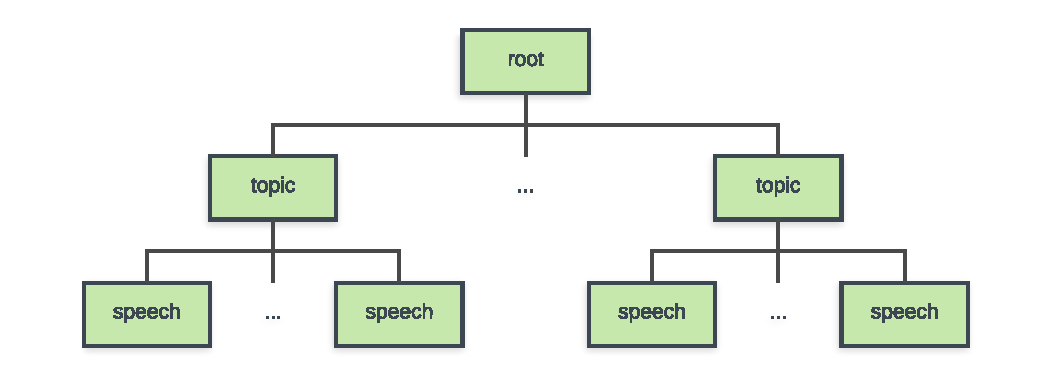
\includegraphics[width=\textwidth]{figures/tree.pdf}
  \caption{The structure of a parliamentary debate is that of a shallow
    tree.\label{fig:tree}}
\end{figure}

The common ways to do sentence classification (e.g.\ convolutional neural
networks \citep{kim2014conv}, recurrent neural networks or the simpler
bag-of-words models) operate on sentences in a vacuum, considering only their
linguistic contents and ignoring any contextual information that might be
contained in the layout in which the text might have been embedded. This is to
be expected considering that most of the common datasets in this area really
\emph{are} just small bits of text in a vacuum; often-used datasets involve
Twitter messages or short product reviews. In this case however, the sentences
come from a document with a rich structure providing a lot of context.
Anecdotally, as a human it is trivial to discern section headers in a document
even when the document is in a foreign language; simply the fact that the
section header might be printed in bold and centered rather than left-aligned
gives it away.  Incorporating this structural data into the learning process,
using a clustering approach inspired by \textcite{klampfl2014unsupervised},
will hopefully increase the performance of the system, either by simply scoring
better on the used metrics, or perhaps more indirectly by requiring less data or
training time to achieve the same score.

%%% Local Variables:
%%% mode: latex
%%% TeX-master: "report"
%%% End:
